\documentclass[convert={ghostscript,gsdevice=tiffg4,
outext=.tiff,density=1200}]{standalone}
    \usepackage{tikz}
    \usepackage{pgfplots}
    \usetikzlibrary{patterns}

\begin{document}
\Large
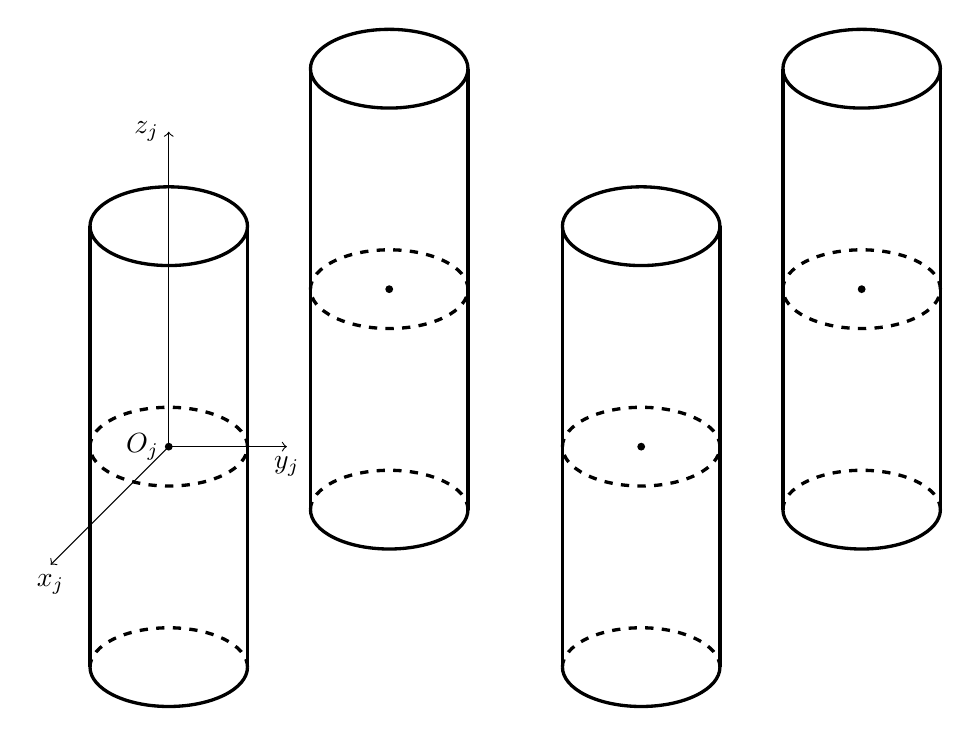
\begin{tikzpicture}
  \draw[->] (0,0) -- (1.5,0) node[anchor=north] {$y_j$};
  \draw[->] (0,0) -- (0,4) node[anchor=east] {$z_j$};
  \draw[->] (0,0) -- (-1.5,-1.5) node[anchor=north] {$x_j$};

  \node[left] at (0,0) {$O_j$};

  \draw[very thick, dashed] (0,0) ellipse (1.0 and .5);
  \draw[very thick] (0,2.8) ellipse (1.0 and .5);
  \draw[very thick] (-1.0,-2.8) arc (180:360:1.0 and .5);
  \draw[very thick, dashed] (1.0,-2.8) arc (0:180:1.0 and .5);
  \draw[very thick] (-1.0,-2.8) -- (-1.0,2.8);
  \draw[very thick] (1.0,-2.8) -- (1.0,2.8);

  \draw[very thick, dashed] (2.8,2) ellipse (1.0 and .5);
  \draw[very thick] (2.8,4.8) ellipse (1.0 and .5);
  \draw[very thick] (1.8,-0.8) arc (180:360:1.0 and .5);
  \draw[very thick, dashed] (3.8,-0.8) arc (0:180:1.0 and .5);
  \draw[very thick] (1.8,-0.8) -- (1.8,4.8);
  \draw[very thick] (3.8,-0.8) -- (3.8,4.8);

  \draw[very thick, dashed] (6,0) ellipse (1.0 and .5);
  \draw[very thick] (6,2.8) ellipse (1.0 and .5);
  \draw[very thick] (5.0,-2.8) arc (180:360:1.0 and .5);
  \draw[very thick, dashed] (7.0,-2.8) arc (0:180:1.0 and .5);
  \draw[very thick] (5.0,-2.8) -- (5.0,2.8);
  \draw[very thick] (7.0,-2.8) -- (7.0,2.8);

  \draw[very thick, dashed] (8.8,2) ellipse (1.0 and .5);
  \draw[very thick] (8.8,4.8) ellipse (1.0 and .5);
  \draw[very thick] (7.8,-0.8) arc (180:360:1.0 and .5);
  \draw[very thick, dashed] (9.8,-0.8) arc (0:180:1.0 and .5);
  \draw[very thick] (7.8,-0.8) -- (7.8,4.8);
  \draw[very thick] (9.8,-0.8) -- (9.8,4.8);


  \node[circle, fill=black, inner sep=1pt] at (0,0) {};
  \node[circle, fill=black, inner sep=1pt] at (2.8,2) {};
  \node[circle, fill=black, inner sep=1pt] at (6,0) {};
  \node[circle, fill=black, inner sep=1pt] at (8.8,2) {};

\end{tikzpicture}
\end{document}

%%% Local Variables: 
%%% mode: latex
%%% TeX-master: t
%%% End: 
